\documentclass[a4paper,12pt,twoside,openany]{report}
%
% Wzorzec pracy dyplomowej
% J. Starzynski (jstar@iem.pw.edu.pl) na podstawie pracy dyplomowej
% mgr. Błażeja Wincenciaka
% Wersja 3.0 - 10 stycznia 2009
%
\usepackage{polski}
\usepackage[utf8]{inputenc}
\usepackage[pdftex]{graphicx}
\usepackage{tabularx}
\usepackage{array}
\usepackage[polish]{babel}
% \usepackage{subfigure}
\usepackage{amsfonts}
\usepackage{verbatim}
\usepackage{indentfirst}
\usepackage[pdftex]{hyperref}


% rozmaite polecenia pomocnicze
% gdzie rysunki?
\newcommand{\ImgPath}{img}

% oznaczenie rzeczy do zrobienia/poprawienia
\newcommand{\TODO}{\textbf{TODO}}


% wyroznienie slow kluczowych
\newcommand{\tech}{\texttt}

% na oprawe (1.0cm - 0.7cm)*2 = 0.6cm
% na oprawe (1.1cm - 0.7cm)*2 = 0.8cm
%  oddsidemargin lewy margines na nieparzystych stronach
% evensidemargin lewy margines na parzystych stronach
\def\oprawa{1.05cm}
\addtolength{\oddsidemargin}{\oprawa}
\addtolength{\evensidemargin}{-\oprawa}

% table span multirows
\usepackage{multirow}
\usepackage{enumitem}	% enumitem.pdf
\usepackage[section]{placeins}

\setlist{listparindent=\parindent, parsep=\parskip} % potrzebuje enumitem

%%%%%%%%%%%%%%% Dodatkowe Pakiety %%%%%%%%%%%%%%%%%
\usepackage{prmag}   % definiuje komendy opieku,nrindeksu, rodzaj pracy, ...
\usepackage{pgfplots}
\usepackage{tikz}
\usepackage{subcaption}
%%%%%%%%%%%%%%% Strona Tytułowa %%%%%%%%%%%%%%%%%
\title{Porównanie wydajności serwisów RESTful w wybranych platformach programowania}

\author{Marcin Jasion}
\nrindeksu{230338}
% wstawienie zdjecia
\zdjecie{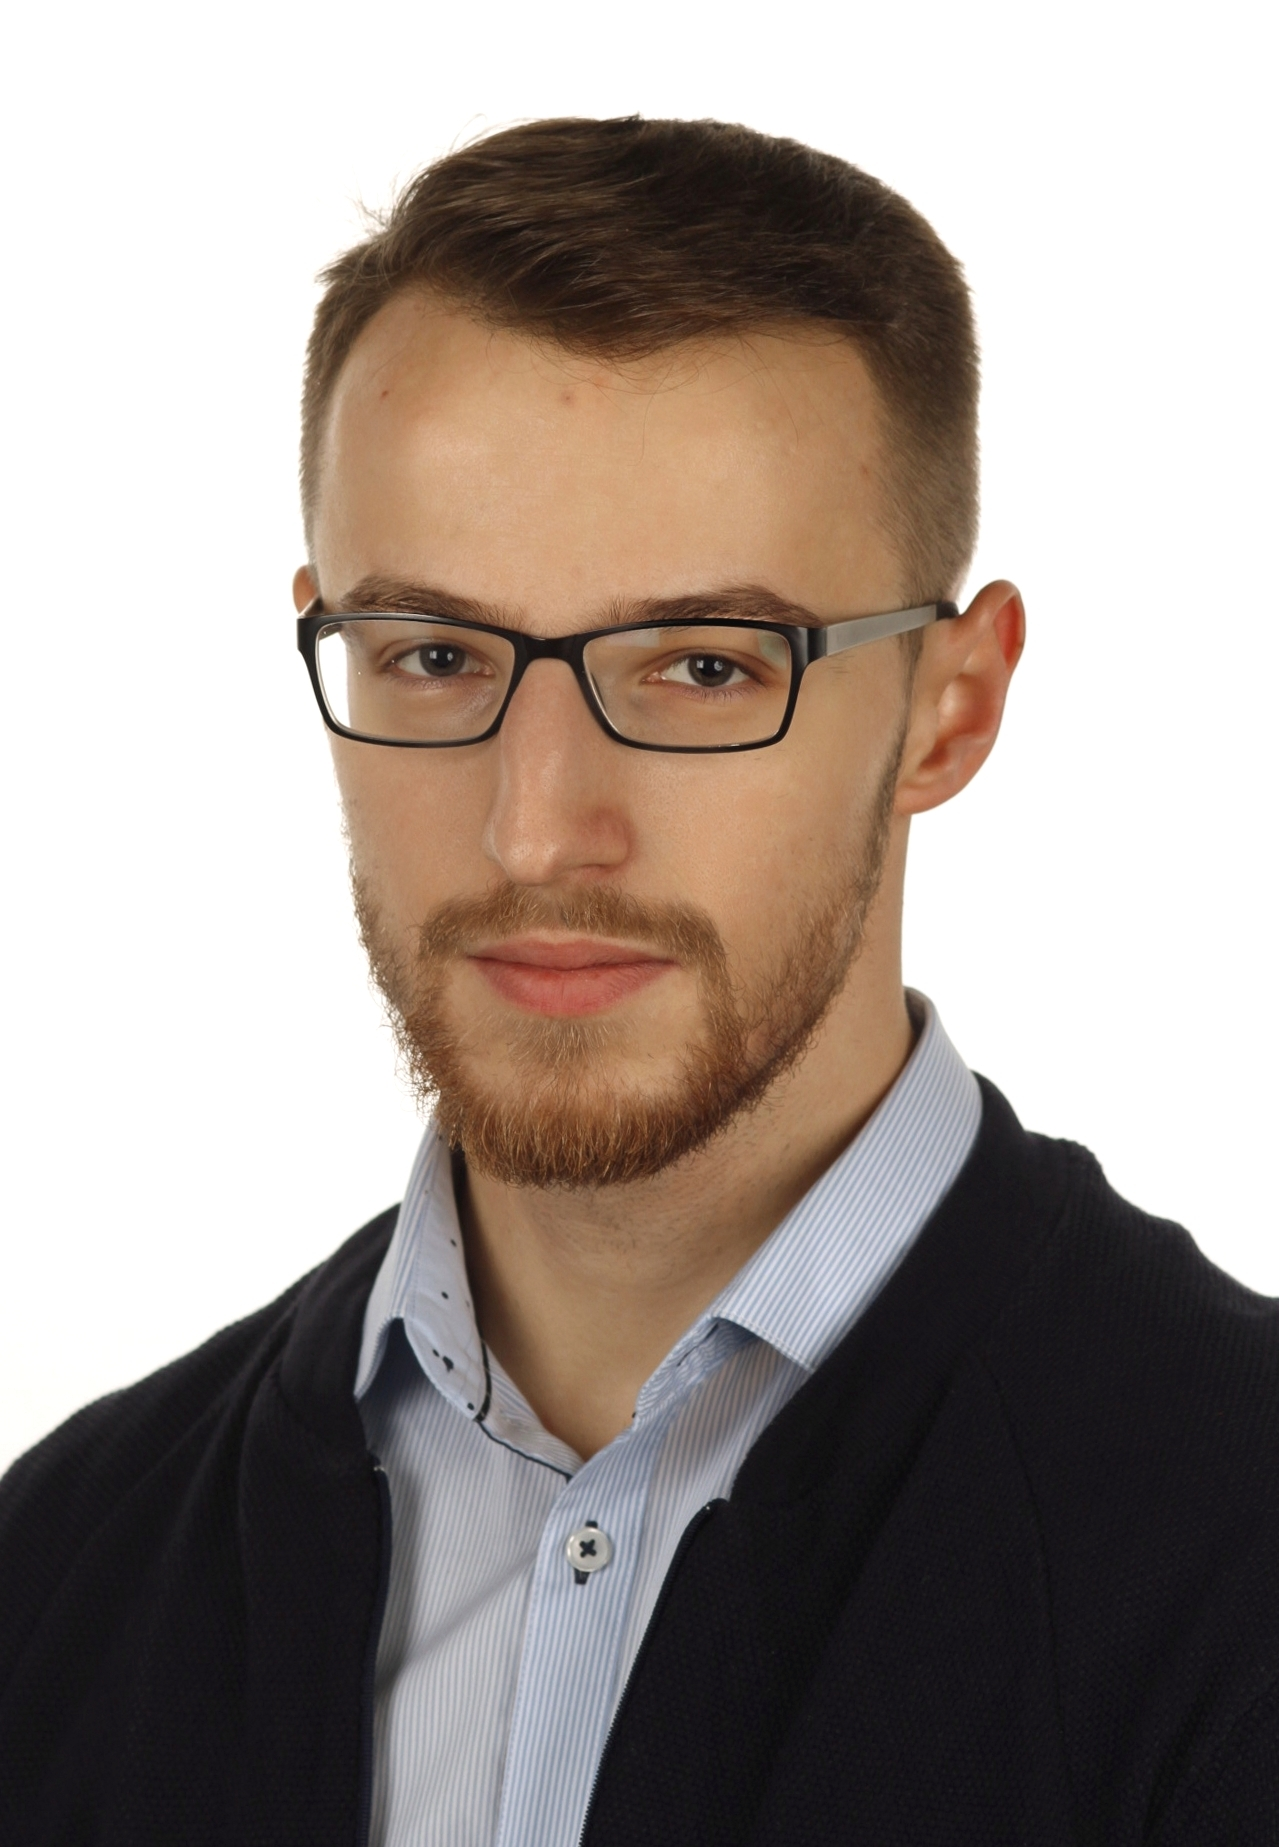
\includegraphics[width=4cm]{\ImgPath/zdjecie_profilowe.jpg}}

\opiekun{prof. nzw. dr hab. inż. Krzysztof Siwek}
\terminwykonania{1 stycznia 1970} % TODO
\datawydaniatematu{1 stycznia 1970} % TODO
\rokakademicki{1970/1970} % TODO

% zakres pracy
\zakres {\begin{enumerate}
 \item Przegląd istniejących rozwiązań
 \item Projekt systemu
 \item Implementacja
 \item Opis testów
 \item Analiza przeprowadzonych testów
\end{enumerate}
}

% Podziekowanie - opcjonalne
% \podziekowania{\noindent
{\Large Podziękowania}
\bigskip

Dziękujemy bardzo serdecznie wszystkim, a w szczególności Rodzinom i~Unii Europejskiej...

\bigskip

{\raggedleft
Zdolny Student i Pracowity Kolega

}

}

\opinie{%
  \newpage
\begin{center}
 {\large\bf  Opinia} \\
\end{center}

  \newpage
  \newpage
\begin{center}
 {\large\bf  Recenzja } 
\end{center}
}

\begin{document}
\maketitle

\chapter{Wstęp}

\chapter{Przegląd literatury}
\section{Serwisy RESTful}
\subsection{Czym jest serwis RESTful}
\subsection{Mikroserwisy}
\section{Java}
\subsection{Historia i ewolucja języka Java}
\subsection{Java 8}
\subsection{Biblioteka Spring}
\subsection{Kontenery aplikacji}
\subsubsection{Tomcat8}
\subsubsection{Jetty9}

\section{Go}
\subsection{Historia i ewolucja języka Go}
\subsection{Biblioteka mgo}

\chapter{Narzędzia wykorzystane do przeprowadzenia testów}
\section{Docker}
\section{MongoDB}
\section{Apache JMeter}
\section{Digitalocean}
\chapter{Projekt Aplikacji}
\section{Opis}
Aplikacja stworzona na potrzeby przeprowadzenia badań jest serwisem typu \textsl{RESTful}. Celem jest przechowywanie danych w bazie w postaci klucz-wartość.  Aplikacja udostępnia w tym celu \textsl{API}. Aby móc skorzystać z aplikacji klient musi się autoryzować unikalnym kluczem (\textsl{API key}). Klient posiadający klucz ma możliwość zapisywać i odczytywać dane. 

Klucz można otrzymać automatycznie wykonując żądanie: \textsl{GET /api/}. W odpowiedzi aplikacja zwróci unikalny, losowy klucz identyfikujący danego klienta. Do generowania kluczy użyty został mechanizm \textsl{UUID} (ang. \textsl{universally unique identifier}) generujący losowy 128 bitowy ciąg znaków. Przykładowy identyfikator wygląda następująco: \textsl{f0778bae-2902-4ff6-93fa-9776403ecb0f}.

Klient posiadający swój klucz może tworzyć, aktualizować, usuwać i pobierać wartości które są zapisane w bazie danych. Każde żądanie w adresie musi w adresie zawierać ten klucz. Początek żądania ma formę \textsl{/api/\{api\_key\}/}. W przypadku podania błędnego klucza lub jego braku aplikacja zwróci błąd autoryzacji. W tabeli \ref{tab:restcache-api} zostały zaprezentowane dostępne metody, do zarządzania danymi.
\begin{table}[!htb]
\centering
\caption{Metody dostępne w API aplikacji dla klienta}
\label{tab:restcache-api}
\begin{tabularx}{\textwidth}{@{} X X @{}}
\toprule
\multicolumn{1}{c}{\textbf{Żądanie HTTP}}            & \multicolumn{1}{c}{\textbf{Krótki opis}}                                               \\ \midrule
GET /api/\{api\_key\}/\{key\}                        & Pobranie obiektu z bazy znajdującego się pod kluczem \textsl\{key\}                   \\
POST /api/\{api\_key\}/\{key\}                       & Utworzenie obiektu w bazie pod kluczem \textsl\{key\}                                 \\
PUT /api/\{api\_key\}/\{key\}                        & Aktualizowanie obiektu w bazie, znajdującego się pod kluczem \textsl\{key\}        \\
DELETE /api/\{api\_key\}/\{key\} & Usunięcie elementu z bazy elementu o kluczu \textsl\{key\}                            \\
GET /api/\{api\_key\}                                & Pobranie wszystkich obiektów zapisanych w bazie, przypisanych kluczowi \textsl\{API\} \\
\end{tabularx}
\end{table}

Każda z metod służąca do modyfikowania danych ma zaimplementowane odpowiednie walidacje. Meetoda \textsl{} pozwala na pobranie zapisanej wartości w bazie danych. Jeśli nie istnieje wartość o podanym kluczu zwracany jest błąd \textsl{HTTP 404 - Not Found}. Następną metodą umożliwia tworzyć obiekty w bazie danych. Jeśli w bazie istnieje już obiekt o podanym kluczu, przypisany temu samemu klientowi aplikacja zwraca błąd \textsl{HTTP 409 - Conflict}.f

Ostatnią dostępną metodą jest żądanie \textsl{GET /api/\{api\_key\}}, które pozwala na pobranie wszystkich elementów z bazy danych. Je

Model wykorzystywany w aplikacji składa z dwóch klas które są jednakowo odwzorowane w kolekcjach bazy \textsl{MongoDB}. Klasa \textsl{Api} służy do przechowywania w bazie danych informacji o zarejestrowanych kluczach API (\textsl{API key}). Jeśli w kolekcji \textsl{Api} nie występuje klucz, aplikacja będzie zgłaszać błąd braku autoryzacji. Druga klasa, \textsl{Cache}, jest obiektem służącym do przechowywania.

Na rysunku \ref{fig:class_diagram} przedstawiony jest diagram klas aplikacji. 
\begin{figure}[!ht]
\centering
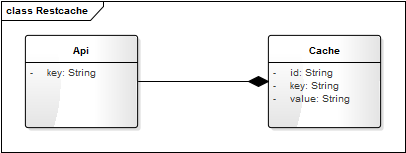
\includegraphics[width=13cm]{\ImgPath/diagram_klas.png}
\caption{Diagram klas aplikacji wykorzystywanej do przeprowadzenia testów}
\label{fig:class_diagram}
\end{figure}

\subsection{Infrastruktura}
Do przeprowadzenia testów wydajnościowych wykorzystywane były 3 serwery wirtualne. Specyfikacje techniczne serwerów wirtualnych, wykorzystanych w testach to: 
\begin{itemize}
    \item 8 rdzeni, 16 gigabajtów pamięci RAM, 160 gigabajtów dysku SSD dla serwera aplikacyjnego
    \item 4 rdzenie, 8 gigabajtów pamięci RAM, 80 gigabajtów dysku SSD dla serwera bazy danych 
    \item 4 rdzenie, 8 gigabajtów pamięci RAM, 80 gigabajtów dysku SSD dla serwera, na którym uruchomiony był program \textsl{Apache JMeter}
\end{itemize}
Serwery komunikowały się po sieci lokalnej (ang. \textsl{LAN}) bezpośrednio między sobą.

Na rysunku \ref{fig:deployment_diagram} zaprezentowany został diagram wdrożenia infrastruktury wykorzystanej do przeprowadzenia testóœ.
\begin{figure}[!ht]
\centering
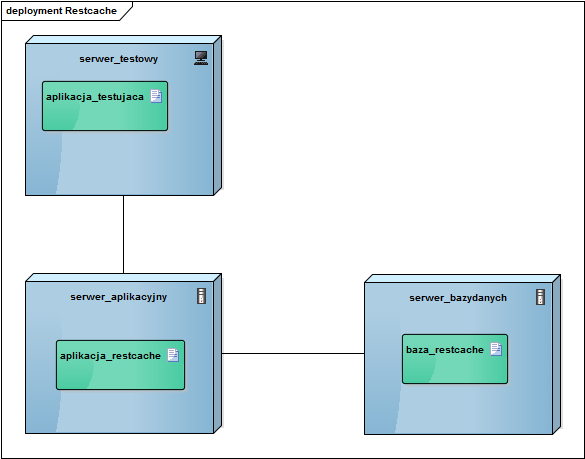
\includegraphics[width=13cm]{\ImgPath/diagram_wdrozenia.png}
\caption{Diagram wdrożenia infrastruktury wykorzystywanej do przeprowadzenia testów}
\label{fig:deployment_diagram}
\end{figure}

\subsection{Testy akceptacyjne} 

By potwierdzić, że \textsl{API} aplikacji w językach \textsl{Java} i \textsl{Go} jest zachowuje się tak samo zostało przygotowane 24 testy akceptacyjnych używając biblioteki \textsl{Spock}. 

W dodatku \ref{sec:acceptance_tests_appendix} przedstawione zostały rezultaty testów aplikacji uruchomionej na serwerze \textsl{Tomcat} (rysunek \ref{fig:acceptance_test_tomcat}), \textsl{Jetty} (rysunek \ref{fig:acceptance_test_jetty}) oraz w języku \textsl{Go} (rysunek \ref{fig:acceptance_test_go}).



\chapter{Testy wydajnościowe}
\section{Środowisko testowe}
\section{Opis testów}
\section{Wyniki testów - pusta baza danych}

\newpage
\subsection{Testy wydajności walidacji API}
\pgfplotsset{grid style={dashed}}
\begin{figure}[!ht]
\captionsetup[subfigure]{singlelinecheck=off, justification=centering}
\showcaptionsetup{subfigure}
\hspace{-2.5cm}
\begin{subfigure}{0.5\textwidth}
\pgfplotstableread[col sep = comma]{csv_queries/requests_per_sec/tomcat_clean_api_validation.csv}\csvdata
\begin{tikzpicture}
  \begin{axis}[xmin = 0, xmax=900, ymin = 0, scaled y ticks = base 10:-3, xlabel = {Czas [s]}, ylabel = Liczba żądań, legend pos=south east, ymajorgrids] %TODO miary?
    \addplot[color=blue,mark=none] table[x index=0, y index=1]{\csvdata};
    \addplot[color=green,mark=none] table[x index=0, y index=2]{\csvdata};
    \legend{100,250}
  \end{axis}
\end{tikzpicture}
\caption{Tomcat 8 - liczba żądań obsłużonych przez aplikację w ciągu sekundy}
\label{fig:tomcat_clean_api_validation_rps}
\end{subfigure}

\hspace{3cm}
\begin{subfigure}{0.5\textwidth}
\pgfplotstableread[col sep = comma]{csv_queries/response_time_distribution/tomcat_clean_api_validation_100.csv}\csva
\pgfplotstableread[col sep = comma]{csv_queries/response_time_distribution/tomcat_clean_api_validation_250.csv}\csvb
\pgfplotsset{
    /pgfplots/ybar legend/.style={
    /pgfplots/legend image code/.code={\draw[##1,/tikz/.cd,yshift=-0.25em](0cm,0cm) rectangle(1pt,0.7em);},
   }
}
\begin{tikzpicture}
  \begin{axis}[ybar, bar width=0.5, xmin = 0, ymin = 0, scaled y ticks = base 10:-5, xlabel = {Czas odpowiedzi [ms]}, ylabel = {Liczba żądań}, ymajorgrids] %TODO miary?
    \addplot[color=blue, mark=none, fill=blue] table[x index=0, y index=1]{\csva};
    \addplot[color=green, mark=none, fill=green] table[x index=0, y index=1]{\csvb};
    \legend{100,250}
  \end{axis}
\end{tikzpicture}
\caption{Tomcat 8 - rozkład czasów odpowiedzi aplikacji (95\% odpowiedzi)}
\label{fig:tomcat_clean_api_validation_td}
\end{subfigure}

\caption{Tomcat 8 - testy wydajności walidacji istnienia klucza API}
\label{fig:tomcat_clean_api_validation}
\end{figure}

\clearpage
\pgfplotsset{grid style={dashed}}
\begin{figure}[!ht]
\captionsetup[subfigure]{singlelinecheck=off, justification=centering}
\showcaptionsetup{subfigure}
\hspace{-2.5cm}
\begin{subfigure}{0.5\textwidth}
\pgfplotstableread[col sep = comma]{csv_queries/requests_per_sec/jetty_clean_api_validation.csv}\csvdata
\begin{tikzpicture}
  \begin{axis}[xmin = 0, xmax=900, ymin = 0, scaled y ticks = base 10:-3, xlabel = {Czas [s]}, ylabel = Liczba żądań, legend pos=south east, ymajorgrids] %TODO miary?
    \addplot[color=blue,mark=none] table[x index=0, y index=1]{\csvdata};
    \addplot[color=green,mark=none] table[x index=0, y index=2]{\csvdata};
    \legend{100,250}
  \end{axis}
\end{tikzpicture}
\caption{Jetty 9 - liczba żądań obsłużonych przez aplikację w ciągu sekundy}
\label{fig:jetty_clean_api_validation_rps}
\end{subfigure}

\hspace{3cm}
\begin{subfigure}{0.5\textwidth}
\pgfplotstableread[col sep = comma]{csv_queries/response_time_distribution/jetty_clean_api_validation_100.csv}\csva
\pgfplotstableread[col sep = comma]{csv_queries/response_time_distribution/jetty_clean_api_validation_250.csv}\csvb
\pgfplotsset{
    /pgfplots/ybar legend/.style={
    /pgfplots/legend image code/.code={\draw[##1,/tikz/.cd,yshift=-0.25em](0cm,0cm) rectangle(1pt,0.7em);},
   }
}
\begin{tikzpicture}
  \begin{axis}[ybar, bar width=0.5, xmin = 0, ymin = 0, scaled y ticks = base 10:-5, xlabel = {Czas odpowiedzi [ms]}, ylabel = {Liczba żądań}, ymajorgrids] %TODO miary?
    \addplot[color=blue, mark=none, fill=blue] table[x index=0, y index=1]{\csva};
    \addplot[color=green, mark=none, fill=green] table[x index=0, y index=1]{\csvb};
    \legend{100,250}
  \end{axis}
\end{tikzpicture}
\caption{Jetty 9 - rozkład czasów odpowiedzi aplikacji (95\% odpowiedzi)}
\label{fig:jetty_clean_api_validation_td}
\end{subfigure}

\caption{Jetty 9 - testy wydajności walidacji istnienia klucza API}
\label{fig:jetty_clean_api_validation}
\end{figure}

\clearpage
\pgfplotsset{grid style={dashed}}
\begin{figure}[!ht]
\captionsetup[subfigure]{singlelinecheck=off, justification=centering}
\showcaptionsetup{subfigure}
\hspace{-2.5cm}
\begin{subfigure}{0.5\textwidth}
\pgfplotstableread[col sep = comma]{csv_queries/requests_per_sec/go_clean_api_validation.csv}\csvdata
\begin{tikzpicture}
  \begin{axis}[xmin = 0, xmax=900, ymin = 0, scaled y ticks = base 10:-3, xlabel = {Czas [s]}, ylabel = Liczba żądań, legend pos=south east, ymajorgrids] %TODO miary?
    \addplot[color=blue,mark=none] table[x index=0, y index=1]{\csvdata};
    \addplot[color=green,mark=none] table[x index=0, y index=2]{\csvdata};
    \legend{100,250}
  \end{axis}
\end{tikzpicture}
\caption{Go - liczba żądań obsłużonych przez aplikację w ciągu sekundy}
\label{fig:go_clean_api_validation_rps}
\end{subfigure}

\hspace{3cm}
\begin{subfigure}{0.5\textwidth}
\pgfplotstableread[col sep = comma]{csv_queries/response_time_distribution/go_clean_api_validation_100.csv}\csva
\pgfplotstableread[col sep = comma]{csv_queries/response_time_distribution/go_clean_api_validation_250.csv}\csvb
\pgfplotsset{
    /pgfplots/ybar legend/.style={
    /pgfplots/legend image code/.code={\draw[##1,/tikz/.cd,yshift=-0.25em](0cm,0cm) rectangle(1pt,0.7em);},
   }
}
\begin{tikzpicture}
  \begin{axis}[ybar, bar width=0.5, xmin = 0, ymin = 0, scaled y ticks = base 10:-5, xlabel = {Czas odpowiedzi [ms]}, ylabel = {Liczba żądań}, ymajorgrids] %TODO miary?
    \addplot[color=blue, mark=none, fill=blue] table[x index=0, y index=1]{\csva};
    \addplot[color=green, mark=none, fill=green] table[x index=0, y index=1]{\csvb};
    \legend{100,250}
  \end{axis}
\end{tikzpicture}
\caption{Go - rozkład czasów odpowiedzi aplikacji (95\% odpowiedzi)}
\label{fig:go_clean_api_validation_td}
\end{subfigure}

\caption{Go - testy wydajności walidacji istnienia klucza API}
\label{fig:go_clean_api_validation}
\end{figure}

\clearpage

\clearpage

\begin{table}[!htb]
\centering
\caption{Wykorzystanie procesora i pamięci RAM na serwerze, gdzie uruchomiona była aplikacja}
\label{tab:app-clean-api}
\begin{tabular}{@{}ccccl@{}}
\toprule
\textbf{Język} & \textbf{Liczba wątków} & \multicolumn{1}{p{3cm}}{\textbf{Średnie wykorzystanie CPU (\%)}} & \multicolumn{1}{p{3cm}}{\textbf{Średnie wykorzystanie RAM (MB)}} &  \\ \midrule
Tomcat 8       & 100                    & 77.50                             & 1882.60                          &  \\
Tomcat 8       & 250                    & 65.73                             & 1926.08                          &  \\
Jetty 9       & 100                    & 70.13                             & 2020.03                          &  \\
Jetty 9       & 250                    & 59.31                             & 2005.06                          &  \\
Go       & 100                    & 29.93                             & 211.65                          &  \\
Go       & 250                    & 31.64                             & 228.72                          &  \\
\bottomrule
\end{tabular}
\end{table}

\begin{table}[!htb]
\centering
\caption{Wykorzystanie procesora i pamięci RAM na serwerze, gdzie uruchomiona była baza danych MongoDB}
\label{tab:mongo-clean-api}
\begin{tabular}{@{}ccccl@{}}
\toprule
\textbf{Język} & \textbf{Liczba wątków} & \multicolumn{1}{p{3cm}}{\textbf{Średnie wykorzystanie CPU (\%)}} & \multicolumn{1}{p{3cm}}{\textbf{Średnie wykorzystanie RAM (MB)}} &  \\ \midrule
Tomcat 8       & 100                    & 29.4                             & 151.1                          &  \\
Tomcat 8       & 250                    & 22.05                             & 272.9                          &  \\
Jetty 9       & 100                    & 30.29                             & 301.42                          &  \\
Jetty 9       & 250                    & 22.55                             & 270.23                          &  \\
Go       & 100                    & 18.92                             & 302.67                          &  \\
Go       & 250                    & 16.84                             & 358.49                          &  \\
\bottomrule
\end{tabular}
\end{table}

 \newpage
 \subsection{Test wydajności walidacji kluczy w bazie}
\pgfplotsset{grid style={dashed}}
\begin{figure}[!ht]
\pgfplotstableread[col sep = comma]{csv_queries/requests_per_sec/tomcat_clean_key_validation.csv}\csvdata
\begin{tikzpicture}
  \begin{axis}[xmin = 0, xmax=900, ymin = 0, scaled y ticks = base 10:-3, xlabel = {Czas [s]}, ylabel = Liczba żądań, legend pos=south east, ymajorgrids] %TODO miary?
    \addplot[color=blue,mark=none] table[x index=0, y index=1]{\csvdata};
    \addplot[color=green,mark=none] table[x index=0, y index=2]{\csvdata};
    \legend{100,250}
  \end{axis}
\end{tikzpicture}
\caption{Tomcat 8 - liczba żądań obsłużonych przez aplikację w ciągu sekundy podczas testu walidacji istnienia rekordu w bazie}
\label{fig:tomcat_clean_key_validation_rps}
\end{figure}

\begin{figure}[!ht]
\pgfplotstableread[col sep = comma]{csv_queries/response_time_distribution/tomcat_clean_key_validation_100.csv}\csva
\pgfplotstableread[col sep = comma]{csv_queries/response_time_distribution/tomcat_clean_key_validation_250.csv}\csvb
\pgfplotsset{
    /pgfplots/ybar legend/.style={
    /pgfplots/legend image code/.code={\draw[##1,/tikz/.cd,yshift=-0.25em](0cm,0cm) rectangle(1pt,0.7em);},
   }
}
\begin{tikzpicture}
  \begin{axis}[ybar, bar width=0.5, xmin = 0, ymin = 0, scaled y ticks = base 10:-5, xlabel = {Czas odpowiedzi [ms]}, ylabel = {Liczba żądań}, ymajorgrids] %TODO miary?
    \addplot[color=blue, mark=none, fill=blue] table[x index=0, y index=1]{\csva};
    \addplot[color=green, mark=none, fill=green] table[x index=0, y index=1]{\csvb};
    \legend{100,250}
  \end{axis}
\end{tikzpicture}
\caption{Tomcat 8 - rozkład czasów odpowiedzi aplikacji (95\% odpowiedzi) podczas testu walidacji istnienia rekordu w bazie}
\label{fig:tomcat_clean_key_validation_td}
\end{figure}

\pgfplotsset{grid style={dashed}}
\begin{figure}[!ht]
\pgfplotstableread[col sep = comma]{csv_queries/requests_per_sec/jetty_clean_key_validation.csv}\csvdata
\begin{tikzpicture}
  \begin{axis}[xmin = 0, xmax=900, ymin = 0, scaled y ticks = base 10:-3, xlabel = {Czas [s]}, ylabel = Liczba żądań, legend pos=south east, ymajorgrids] %TODO miary?
    \addplot[color=blue,mark=none] table[x index=0, y index=1]{\csvdata};
    \addplot[color=green,mark=none] table[x index=0, y index=2]{\csvdata};
    \legend{100,250}
  \end{axis}
\end{tikzpicture}
\caption{Jetty 9 - liczba żądań obsłużonych przez aplikację w ciągu sekundy podczas testu walidacji istnienia rekordu w bazie}
\label{fig:jetty_clean_key_validation_rps}
\end{figure}

\begin{figure}[!ht]
\pgfplotstableread[col sep = comma]{csv_queries/response_time_distribution/jetty_clean_key_validation_100.csv}\csva
\pgfplotstableread[col sep = comma]{csv_queries/response_time_distribution/jetty_clean_key_validation_250.csv}\csvb
\pgfplotsset{
    /pgfplots/ybar legend/.style={
    /pgfplots/legend image code/.code={\draw[##1,/tikz/.cd,yshift=-0.25em](0cm,0cm) rectangle(1pt,0.7em);},
   }
}
\begin{tikzpicture}
  \begin{axis}[ybar, bar width=0.5, xmin = 0, ymin = 0, scaled y ticks = base 10:-5, xlabel = {Czas odpowiedzi [ms]}, ylabel = {Liczba żądań}, ymajorgrids] %TODO miary?
    \addplot[color=blue, mark=none, fill=blue] table[x index=0, y index=1]{\csva};
    \addplot[color=green, mark=none, fill=green] table[x index=0, y index=1]{\csvb};
    \legend{100,250}
  \end{axis}
\end{tikzpicture}
\caption{Jetty 9 - rozkład czasów odpowiedzi aplikacji (95\% odpowiedzi) podczas testu walidacji istnienia rekordu w bazie}
\label{fig:jetty_clean_key_validation_td}
\end{figure}

\pgfplotsset{grid style={dashed}}
\begin{figure}[!ht]
\pgfplotstableread[col sep = comma]{csv_queries/requests_per_sec/go_clean_key_validation.csv}\csvdata
\begin{tikzpicture}
  \begin{axis}[xmin = 0, xmax=900, ymin = 0, scaled y ticks = base 10:-3, xlabel = {Czas [s]}, ylabel = Liczba żądań, legend pos=south east, ymajorgrids] %TODO miary?
    \addplot[color=blue,mark=none] table[x index=0, y index=1]{\csvdata};
    \addplot[color=green,mark=none] table[x index=0, y index=2]{\csvdata};
    \legend{100,250}
  \end{axis}
\end{tikzpicture}
\caption{Go - liczba żądań obsłużonych przez aplikację w ciągu sekundy podczas testu walidacji istnienia rekordu w bazie}
\label{fig:go_clean_key_validation_rps}
\end{figure}

\begin{figure}[!ht]
\pgfplotstableread[col sep = comma]{csv_queries/response_time_distribution/go_clean_key_validation_100.csv}\csva
\pgfplotstableread[col sep = comma]{csv_queries/response_time_distribution/go_clean_key_validation_250.csv}\csvb
\pgfplotsset{
    /pgfplots/ybar legend/.style={
    /pgfplots/legend image code/.code={\draw[##1,/tikz/.cd,yshift=-0.25em](0cm,0cm) rectangle(1pt,0.7em);},
   }
}
\begin{tikzpicture}
  \begin{axis}[ybar, bar width=0.5, xmin = 0, ymin = 0, scaled y ticks = base 10:-5, xlabel = {Czas odpowiedzi [ms]}, ylabel = {Liczba żądań}, ymajorgrids] %TODO miary?
    \addplot[color=blue, mark=none, fill=blue] table[x index=0, y index=1]{\csva};
    \addplot[color=green, mark=none, fill=green] table[x index=0, y index=1]{\csvb};
    \legend{100,250}
  \end{axis}
\end{tikzpicture}
\caption{Go - rozkład czasów odpowiedzi aplikacji (95\% odpowiedzi) podczas testu walidacji istnienia rekordu w bazie}
\label{fig:go_clean_key_validation_td}
\end{figure}


 \clearpage

 \begin{table}[!htb]
 \centering
 \caption{Wykorzystanie procesora i pamięci RAM na serwerze, gdzie uruchomiona była aplikacja}
 \label{tab:app-clean-key}
 \begin{tabular}{@{}ccccl@{}}
 \toprule
 \textbf{Język} & \textbf{Liczba wątków} & \multicolumn{1}{p{3cm}}{\textbf{Średnie wykorzystanie CPU (\%)}} & \multicolumn{1}{p{3cm}}{\textbf{Średnie wykorzystanie RAM (MB)}} &  \\ \midrule
 Tomcat 8       & 100                    & 50.63                             & 1935.12                          &  \\
 Tomcat 8       & 250                    & 49.02                             & 2009.8                          &  \\
 Jetty 9       & 100                    & 50.61                             & 1949.84                          &  \\
 Jetty 9       & 250                    & 45.24                             & 1851.88                          &  \\
 Go       & 100                    & 39.28                             & 214.6                          &  \\
 Go       & 250                    & 45.59                             & 234.03                          &  \\
 \bottomrule
 \end{tabular}
 \end{table}


 \begin{table}[!htb]
 \centering
 \caption{Wykorzystanie procesora i pamięci RAM na serwerze, gdzie uruchomiona była baza danych MongoDB}
 \label{tab:mongo-clean-key}
 \begin{tabular}{@{}ccccl@{}}
 \toprule
 \textbf{Język} & \textbf{Liczba wątków} & \multicolumn{1}{p{3cm}}{\textbf{Średnie wykorzystanie CPU (\%)}} & \multicolumn{1}{p{3cm}}{\textbf{Średnie wykorzystanie RAM (MB)}} &  \\ \midrule
 Tomcat 8       & 100                    & 44.74                             & 167.05                          &  \\
 Tomcat 8       & 250                    & 39.64                             & 277.01                          &  \\
 Jetty 9       & 100                    & 58.65                             & 260.65                          &  \\
 Jetty 9       & 250                    & 43.34                             & 268.43                          &  \\
 Go       & 100                    & 42.72                             & 302.94                          &  \\
 Go       & 250                    & 41.54                             & 365.98                          &  \\
 \bottomrule
 \end{tabular}
 \end{table}


 \newpage
 \subsection{Test wydajności operacji CRUD}
\pgfplotsset{grid style={dashed}}
\begin{figure}[!ht]
\pgfplotstableread[col sep = comma]{csv_queries/requests_per_sec/tomcat_clean_crud.csv}\csvdata
\begin{tikzpicture}
  \begin{axis}[xmin = 0, xmax=900, ymin = 0, scaled y ticks = base 10:-3, xlabel = {Czas [s]}, ylabel = Liczba żądań, legend pos=south east, ymajorgrids,width=13cm, height=6cm] %TODO miary?
    \addplot[color=blue,mark=none] table[x index=0, y index=1]{\csvdata};
    \addplot[color=green,mark=none] table[x index=0, y index=2]{\csvdata};
    \legend{100,250}
  \end{axis}
\end{tikzpicture}
\caption{Tomcat 8 - liczba żądań obsłużonych przez aplikację w ciągu sekundy podczas testu operacji CRUD}
\label{fig:tomcat_clean_crud_rps}
\end{figure}

\begin{figure}[!ht]
\pgfplotstableread[col sep = comma]{csv_queries/response_time_distribution/tomcat_clean_crud_100.csv}\csva
\pgfplotstableread[col sep = comma]{csv_queries/response_time_distribution/tomcat_clean_crud_250.csv}\csvb
\pgfplotsset{
    /pgfplots/ybar legend/.style={
    /pgfplots/legend image code/.code={\draw[##1,/tikz/.cd,yshift=-0.25em](0cm,0cm) rectangle(1pt,0.7em);},
   }
}
\begin{tikzpicture}
  \begin{axis}[ybar, bar width=0.5, xmin = 0, ymin = 0, scaled y ticks = base 10:-5, xlabel = {Czas odpowiedzi [ms]}, ylabel = {Liczba żądań}, ymajorgrids,width=13cm, height=6cm] %TODO miary?
    \addplot[color=blue, mark=none, fill=blue] table[x index=0, y index=1]{\csva};
    \addplot[color=green, mark=none, fill=green] table[x index=0, y index=1]{\csvb};
    \legend{100,250}
  \end{axis}
\end{tikzpicture}
\caption{Tomcat 8 - rozkład czasów odpowiedzi aplikacji (95\% odpowiedzi) podczas testu operacji CRUD}
\label{fig:tomcat_clean_crud_td}
\end{figure}

\pgfplotsset{grid style={dashed}}
\begin{figure}[!ht]
\pgfplotstableread[col sep = comma]{csv_queries/requests_per_sec/jetty_clean_crud.csv}\csvdata
\begin{tikzpicture}
  \begin{axis}[xmin = 0, xmax=900, ymin = 0, scaled y ticks = base 10:-3, xlabel = {Czas [s]}, ylabel = Liczba żądań, legend pos=south east, ymajorgrids,width=13cm, height=6cm] %TODO miary?
    \addplot[color=blue,mark=none] table[x index=0, y index=1]{\csvdata};
    \addplot[color=green,mark=none] table[x index=0, y index=2]{\csvdata};
    \legend{100,250}
  \end{axis}
\end{tikzpicture}
\caption{Jetty 9 - liczba żądań obsłużonych przez aplikację w ciągu sekundy podczas testu operacji CRUD}
\label{fig:jetty_clean_crud_rps}
\end{figure}

\begin{figure}[!ht]
\pgfplotstableread[col sep = comma]{csv_queries/response_time_distribution/jetty_clean_crud_100.csv}\csva
\pgfplotstableread[col sep = comma]{csv_queries/response_time_distribution/jetty_clean_crud_250.csv}\csvb
\pgfplotsset{
    /pgfplots/ybar legend/.style={
    /pgfplots/legend image code/.code={\draw[##1,/tikz/.cd,yshift=-0.25em](0cm,0cm) rectangle(1pt,0.7em);},
   }
}
\begin{tikzpicture}
  \begin{axis}[ybar, bar width=0.5, xmin = 0, ymin = 0, scaled y ticks = base 10:-5, xlabel = {Czas odpowiedzi [ms]}, ylabel = {Liczba żądań}, ymajorgrids,width=13cm, height=6cm] %TODO miary?
    \addplot[color=blue, mark=none, fill=blue] table[x index=0, y index=1]{\csva};
    \addplot[color=green, mark=none, fill=green] table[x index=0, y index=1]{\csvb};
    \legend{100,250}
  \end{axis}
\end{tikzpicture}
\caption{Jetty 9 - rozkład czasów odpowiedzi aplikacji (95\% odpowiedzi) podczas testu operacji CRUD}
\label{fig:jetty_clean_crud_td}
\end{figure}

\pgfplotsset{grid style={dashed}}
\begin{figure}[!ht]
\pgfplotstableread[col sep = comma]{csv_queries/requests_per_sec/go_clean_crud.csv}\csvdata
\begin{tikzpicture}
  \begin{axis}[xmin = 0, xmax=900, ymin = 0, scaled y ticks = base 10:-3, xlabel = {Czas [s]}, ylabel = Liczba żądań, legend pos=south east, ymajorgrids,width=13cm, height=6cm] %TODO miary?
    \addplot[color=blue,mark=none] table[x index=0, y index=1]{\csvdata};
    \addplot[color=green,mark=none] table[x index=0, y index=2]{\csvdata};
    \legend{100,250}
  \end{axis}
\end{tikzpicture}
\caption{Go - liczba żądań obsłużonych przez aplikację w ciągu sekundy podczas testu operacji CRUD}
\label{fig:go_clean_crud_rps}
\end{figure}

\begin{figure}[!ht]
\pgfplotstableread[col sep = comma]{csv_queries/response_time_distribution/go_clean_crud_100.csv}\csva
\pgfplotstableread[col sep = comma]{csv_queries/response_time_distribution/go_clean_crud_250.csv}\csvb
\pgfplotsset{
    /pgfplots/ybar legend/.style={
    /pgfplots/legend image code/.code={\draw[##1,/tikz/.cd,yshift=-0.25em](0cm,0cm) rectangle(1pt,0.7em);},
   }
}
\begin{tikzpicture}
  \begin{axis}[ybar, bar width=0.5, xmin = 0, ymin = 0, scaled y ticks = base 10:-5, xlabel = {Czas odpowiedzi [ms]}, ylabel = {Liczba żądań}, ymajorgrids,width=13cm, height=6cm] %TODO miary?
    \addplot[color=blue, mark=none, fill=blue] table[x index=0, y index=1]{\csva};
    \addplot[color=green, mark=none, fill=green] table[x index=0, y index=1]{\csvb};
    \legend{100,250}
  \end{axis}
\end{tikzpicture}
\caption{Go - rozkład czasów odpowiedzi aplikacji (95\% odpowiedzi) podczas testu operacji CRUD}
\label{fig:go_clean_crud_td}
\end{figure}


 \clearpage

\begin{table}[!htb]
\centering
\caption{Wykorzystanie procesora i pamięci RAM na serwerze, gdzie uruchomiona była aplikacja}
\label{tab:app-clean-crud}
\begin{tabular}{@{}ccccl@{}}
\toprule
\textbf{Język} & \textbf{Liczba wątków} & \multicolumn{1}{p{3cm}}{\textbf{Średnie wykorzystanie CPU (\%)}} & \multicolumn{1}{p{3cm}}{\textbf{Średnie wykorzystanie RAM (MB)}} &  \\ \midrule
Tomcat 8       & 100                    & 42.38                             & 1959.11                          &  \\
Tomcat 8       & 250                    & 40.25                             & 2034.83                          &  \\
Jetty 9       & 100                    & 36.32                             & 1753.27                          &  \\
Jetty 9       & 250                    & 39.6                             & 1605.56                          &  \\
Go       & 100                    & 33.31                             & 222.13                          &  \\
Go       & 250                    & 41.36                             & 242.23                          &  \\
\bottomrule
\end{tabular}
\end{table}


\begin{table}[!htb]
\centering
\caption{Wykorzystanie procesora i pamięci RAM na serwerze, gdzie uruchomiona była baza danych MongoDB}
\label{tab:mongo-clean-crud}
\begin{tabular}{@{}ccccl@{}}
\toprule
\textbf{Język} & \textbf{Liczba wątków} & \multicolumn{1}{p{3cm}}{\textbf{Średnie wykorzystanie CPU (\%)}} & \multicolumn{1}{p{3cm}}{\textbf{Średnie wykorzystanie RAM (MB)}} &  \\ \midrule
Tomcat 8       & 100                    & 59.35                             & 174.04                          &  \\
Tomcat 8       & 250                    & 53.36                             & 276.73                          &  \\
Jetty 9       & 100                    & 59.18                             & 247.87                          &  \\
Jetty 9       & 250                    & 55.55                             & 269.8                          &  \\
Go       & 100                    & 40.46                             & 303.32                          &  \\
Go       & 250                    & 39.74                             & 361.53                          &  \\
\bottomrule
\end{tabular}
\end{table}

 \newpage
 \subsection{Test wydajności walidacji API, walidacji kluczy w bazie oraz operacji CRUD rówlolegle }
\pgfplotsset{grid style={dashed}}
\begin{figure}[!ht]
\pgfplotstableread[col sep = comma]{csv_queries/requests_per_sec/tomcat_clean_all.csv}\csvdata
\begin{tikzpicture}
  \begin{axis}[xmin = 0, xmax=900, ymin = 0, scaled y ticks = base 10:-3, xlabel = {Czas [s]}, ylabel = Liczba żądań, legend pos=south east, ymajorgrids,width=13cm, height=6cm] %TODO miary?
    \addplot[color=blue,mark=none] table[x index=0, y index=1]{\csvdata};
    \addplot[color=green,mark=none] table[x index=0, y index=2]{\csvdata};
    \legend{100,250}
  \end{axis}
\end{tikzpicture}
\caption{Tomcat 8 - liczba żądań obsłużonych przez aplikację w ciągu sekundy podczas testu: walidacji istnienia klucza API, walidacji istnienia, operacji CRUD równolegle}
\label{fig:tomcat_clean_all_rps}
\end{figure}

\begin{figure}[!ht]
\pgfplotstableread[col sep = comma]{csv_queries/response_time_distribution/tomcat_clean_all_100.csv}\csva
\pgfplotstableread[col sep = comma]{csv_queries/response_time_distribution/tomcat_clean_all_250.csv}\csvb
\pgfplotsset{
    /pgfplots/ybar legend/.style={
    /pgfplots/legend image code/.code={\draw[##1,/tikz/.cd,yshift=-0.25em](0cm,0cm) rectangle(1pt,0.7em);},
   }
}
\begin{tikzpicture}
  \begin{axis}[ybar, bar width=0.5, xmin = 0, ymin = 0, scaled y ticks = base 10:-5, xlabel = {Czas odpowiedzi [ms]}, ylabel = {Liczba żądań}, ymajorgrids,width=13cm, height=6cm] %TODO miary?
    \addplot[color=blue, mark=none, fill=blue] table[x index=0, y index=1]{\csva};
    \addplot[color=green, mark=none, fill=green] table[x index=0, y index=1]{\csvb};
    \legend{100,250}
  \end{axis}
\end{tikzpicture}
\caption{Tomcat 8 - rozkład czasów odpowiedzi aplikacji (95\% odpowiedzi) podczas testu: walidacji istnienia klucza API, walidacji istnienia, operacji CRUD równolegle}
\label{fig:tomcat_clean_all_td}
\end{figure}

\pgfplotsset{grid style={dashed}}
\begin{figure}[!ht]
\pgfplotstableread[col sep = comma]{csv_queries/requests_per_sec/jetty_clean_all.csv}\csvdata
\begin{tikzpicture}
  \begin{axis}[xmin = 0, xmax=900, ymin = 0, scaled y ticks = base 10:-3, xlabel = {Czas [s]}, ylabel = Liczba żądań, legend pos=south east, ymajorgrids,width=13cm, height=6cm] %TODO miary?
    \addplot[color=blue,mark=none] table[x index=0, y index=1]{\csvdata};
    \addplot[color=green,mark=none] table[x index=0, y index=2]{\csvdata};
    \legend{100,250}
  \end{axis}
\end{tikzpicture}
\caption{Jetty 9 - liczba żądań obsłużonych przez aplikację w ciągu sekundy podczas testu: walidacji istnienia klucza API, walidacji istnienia, operacji CRUD równolegle}
\label{fig:jetty_clean_all_rps}
\end{figure}

\begin{figure}[!ht]
\pgfplotstableread[col sep = comma]{csv_queries/response_time_distribution/jetty_clean_all_100.csv}\csva
\pgfplotstableread[col sep = comma]{csv_queries/response_time_distribution/jetty_clean_all_250.csv}\csvb
\pgfplotsset{
    /pgfplots/ybar legend/.style={
    /pgfplots/legend image code/.code={\draw[##1,/tikz/.cd,yshift=-0.25em](0cm,0cm) rectangle(1pt,0.7em);},
   }
}
\begin{tikzpicture}
  \begin{axis}[ybar, bar width=0.5, xmin = 0, ymin = 0, scaled y ticks = base 10:-5, xlabel = {Czas odpowiedzi [ms]}, ylabel = {Liczba żądań}, ymajorgrids,width=13cm, height=6cm] %TODO miary?
    \addplot[color=blue, mark=none, fill=blue] table[x index=0, y index=1]{\csva};
    \addplot[color=green, mark=none, fill=green] table[x index=0, y index=1]{\csvb};
    \legend{100,250}
  \end{axis}
\end{tikzpicture}
\caption{Jetty 9 - rozkład czasów odpowiedzi aplikacji (95\% odpowiedzi) podczas testu: walidacji istnienia klucza API, walidacji istnienia, operacji CRUD równolegle}
\label{fig:jetty_clean_all_td}
\end{figure}

\pgfplotsset{grid style={dashed}}
\begin{figure}[!ht]
\pgfplotstableread[col sep = comma]{csv_queries/requests_per_sec/go_clean_all.csv}\csvdata
\begin{tikzpicture}
  \begin{axis}[xmin = 0, xmax=900, ymin = 0, scaled y ticks = base 10:-3, xlabel = {Czas [s]}, ylabel = Liczba żądań, legend pos=south east, ymajorgrids,width=13cm, height=6cm] %TODO miary?
    \addplot[color=blue,mark=none] table[x index=0, y index=1]{\csvdata};
    \addplot[color=green,mark=none] table[x index=0, y index=2]{\csvdata};
    \legend{100,250}
  \end{axis}
\end{tikzpicture}
\caption{Go - liczba żądań obsłużonych przez aplikację w ciągu sekundy podczas testu: walidacji istnienia klucza API, walidacji istnienia, operacji CRUD równolegle}
\label{fig:go_clean_all_rps}
\end{figure}

\begin{figure}[!ht]
\pgfplotstableread[col sep = comma]{csv_queries/response_time_distribution/go_clean_all_100.csv}\csva
\pgfplotstableread[col sep = comma]{csv_queries/response_time_distribution/go_clean_all_250.csv}\csvb
\pgfplotsset{
    /pgfplots/ybar legend/.style={
    /pgfplots/legend image code/.code={\draw[##1,/tikz/.cd,yshift=-0.25em](0cm,0cm) rectangle(1pt,0.7em);},
   }
}
\begin{tikzpicture}
  \begin{axis}[ybar, bar width=0.5, xmin = 0, ymin = 0, scaled y ticks = base 10:-5, xlabel = {Czas odpowiedzi [ms]}, ylabel = {Liczba żądań}, ymajorgrids,width=13cm, height=6cm] %TODO miary?
    \addplot[color=blue, mark=none, fill=blue] table[x index=0, y index=1]{\csva};
    \addplot[color=green, mark=none, fill=green] table[x index=0, y index=1]{\csvb};
    \legend{100,250}
  \end{axis}
\end{tikzpicture}
\caption{Go - rozkład czasów odpowiedzi aplikacji (95\% odpowiedzi) podczas testu: walidacji istnienia klucza API, walidacji istnienia, operacji CRUD równolegle}
\label{fig:go_clean_all_td}
\end{figure}


 \clearpage

 \begin{table}[!htb]
 \centering
 \caption{Wykorzystanie procesora i pamięci RAM na serwerze, gdzie uruchomiona była aplikacja}
 \label{tab:app-clean-all}
 \begin{tabular}{@{}ccccl@{}}
 \toprule
 \textbf{Język} & \textbf{Liczba wątków} & \multicolumn{1}{p{3cm}}{\textbf{Średnie wykorzystanie CPU (\%)}} & \multicolumn{1}{p{3cm}}{\textbf{Średnie wykorzystanie RAM (MB)}} &  \\ \midrule
 Tomcat 8       & 100                    & 56.12                             & 1976.99                          &  \\
 Tomcat 8       & 250                    & 46.62                             & 2063.85                          &  \\
 Jetty 9       & 100                    & 51.55                             & 1944.2                          &  \\
 Jetty 9       & 250                    & 46.04                             & 1600.48                          &  \\
 Go       & 100                    & 40.59                             & 223.55                          &  \\
 Go       & 250                    & 46.66                             & 244.16                          &  \\
 \bottomrule
 \end{tabular}
 \end{table}


 \begin{table}[!htb]
 \centering
 \caption{Wykorzystanie procesora i pamięci RAM na serwerze, gdzie uruchomiona była baza danych MongoDB}
 \label{tab:mongo-clean-all}
 \begin{tabular}{@{}ccccl@{}}
 \toprule
 \textbf{Język} & \textbf{Liczba wątków} & \multicolumn{1}{p{3cm}}{\textbf{Średnie wykorzystanie CPU (\%)}} & \multicolumn{1}{p{3cm}}{\textbf{Średnie wykorzystanie RAM (MB)}} &  \\ \midrule
 Tomcat 8       & 100                    & 55                             & 175.78                          &  \\
 Tomcat 8       & 250                    & 42.89                             & 275.74                          &  \\
 Jetty 9       & 100                    & 61.82                             & 248.13                          &  \\
 Jetty 9       & 250                    & 48.07                             & 269.2                          &  \\
 Go       & 100                    & 41.66                             & 305.38                          &  \\
 Go       & 250                    & 39.77                             & 359.53                          &  \\
 \bottomrule
 \end{tabular}
 \end{table}


 \newpage
 \section{Wyniki testów - baza danych z danymi początkowymi}
 \subsection{Testy wydajności walidacji API}
\pgfplotsset{grid style={dashed}}
\begin{figure}[!ht]
\pgfplotstableread[col sep = comma]{csv_queries/requests_per_sec/tomcat_full_api_validation.csv}\csvdata
\begin{tikzpicture}
  \begin{axis}[xmin = 0, xmax=900, ymin = 0, scaled y ticks = base 10:-3, xlabel = {Czas [s]}, ylabel = Liczba żądań, legend pos=south east, ymajorgrids,width=13cm, height=6cm] %TODO miary?
    \addplot[color=blue,mark=none] table[x index=0, y index=1]{\csvdata};
    \addplot[color=green,mark=none] table[x index=0, y index=2]{\csvdata};
    \legend{100,250}
  \end{axis}
\end{tikzpicture}
\caption{Tomcat 8 - liczba żądań obsłużonych przez aplikację w ciągu sekundy podczas testu walidacji istnienia klucza API}
\label{fig:tomcat_full_api_validation_rps}
\end{figure}

\begin{figure}[!ht]
\pgfplotstableread[col sep = comma]{csv_queries/response_time_distribution/tomcat_full_api_validation_100.csv}\csva
\pgfplotstableread[col sep = comma]{csv_queries/response_time_distribution/tomcat_full_api_validation_250.csv}\csvb
\pgfplotsset{
    /pgfplots/ybar legend/.style={
    /pgfplots/legend image code/.code={\draw[##1,/tikz/.cd,yshift=-0.25em](0cm,0cm) rectangle(1pt,0.7em);},
   }
}
\begin{tikzpicture}
  \begin{axis}[ybar, bar width=0.5, xmin = 0, ymin = 0, scaled y ticks = base 10:-5, xlabel = {Czas odpowiedzi [ms]}, ylabel = {Liczba żądań}, ymajorgrids,width=13cm, height=6cm] %TODO miary?
    \addplot[color=blue, mark=none, fill=blue] table[x index=0, y index=1]{\csva};
    \addplot[color=green, mark=none, fill=green] table[x index=0, y index=1]{\csvb};
    \legend{100,250}
  \end{axis}
\end{tikzpicture}
\caption{Tomcat 8 - rozkład czasów odpowiedzi aplikacji (95\% odpowiedzi) podczas testu walidacji istnienia klucza API}
\label{fig:tomcat_full_api_validation_td}
\end{figure}

\pgfplotsset{grid style={dashed}}
\begin{figure}[!ht]
\pgfplotstableread[col sep = comma]{csv_queries/requests_per_sec/jetty_full_api_validation.csv}\csvdata
\begin{tikzpicture}
  \begin{axis}[xmin = 0, xmax=900, ymin = 0, scaled y ticks = base 10:-3, xlabel = {Czas [s]}, ylabel = Liczba żądań, legend pos=south east, ymajorgrids,width=13cm, height=6cm] %TODO miary?
    \addplot[color=blue,mark=none] table[x index=0, y index=1]{\csvdata};
    \addplot[color=green,mark=none] table[x index=0, y index=2]{\csvdata};
    \legend{100,250}
  \end{axis}
\end{tikzpicture}
\caption{Jetty 9 - liczba żądań obsłużonych przez aplikację w ciągu sekundy podczas testu walidacji istnienia klucza API}
\label{fig:jetty_full_api_validation_rps}
\end{figure}

\begin{figure}[!ht]
\pgfplotstableread[col sep = comma]{csv_queries/response_time_distribution/jetty_full_api_validation_100.csv}\csva
\pgfplotstableread[col sep = comma]{csv_queries/response_time_distribution/jetty_full_api_validation_250.csv}\csvb
\pgfplotsset{
    /pgfplots/ybar legend/.style={
    /pgfplots/legend image code/.code={\draw[##1,/tikz/.cd,yshift=-0.25em](0cm,0cm) rectangle(1pt,0.7em);},
   }
}
\begin{tikzpicture}
  \begin{axis}[ybar, bar width=0.5, xmin = 0, ymin = 0, scaled y ticks = base 10:-5, xlabel = {Czas odpowiedzi [ms]}, ylabel = {Liczba żądań}, ymajorgrids,width=13cm, height=6cm] %TODO miary?
    \addplot[color=blue, mark=none, fill=blue] table[x index=0, y index=1]{\csva};
    \addplot[color=green, mark=none, fill=green] table[x index=0, y index=1]{\csvb};
    \legend{100,250}
  \end{axis}
\end{tikzpicture}
\caption{Jetty 9 - rozkład czasów odpowiedzi aplikacji (95\% odpowiedzi) podczas testu walidacji istnienia klucza API}
\label{fig:jetty_full_api_validation_td}
\end{figure}

\pgfplotsset{grid style={dashed}}
\begin{figure}[!ht]
\pgfplotstableread[col sep = comma]{csv_queries/requests_per_sec/go_full_api_validation.csv}\csvdata
\begin{tikzpicture}
  \begin{axis}[xmin = 0, xmax=900, ymin = 0, scaled y ticks = base 10:-3, xlabel = {Czas [s]}, ylabel = Liczba żądań, legend pos=south east, ymajorgrids,width=13cm, height=6cm] %TODO miary?
    \addplot[color=blue,mark=none] table[x index=0, y index=1]{\csvdata};
    \addplot[color=green,mark=none] table[x index=0, y index=2]{\csvdata};
    \legend{100,250}
  \end{axis}
\end{tikzpicture}
\caption{Go - liczba żądań obsłużonych przez aplikację w ciągu sekundy podczas testu walidacji istnienia klucza API}
\label{fig:go_full_api_validation_rps}
\end{figure}

\begin{figure}[!ht]
\pgfplotstableread[col sep = comma]{csv_queries/response_time_distribution/go_full_api_validation_100.csv}\csva
\pgfplotstableread[col sep = comma]{csv_queries/response_time_distribution/go_full_api_validation_250.csv}\csvb
\pgfplotsset{
    /pgfplots/ybar legend/.style={
    /pgfplots/legend image code/.code={\draw[##1,/tikz/.cd,yshift=-0.25em](0cm,0cm) rectangle(1pt,0.7em);},
   }
}
\begin{tikzpicture}
  \begin{axis}[ybar, bar width=0.5, xmin = 0, ymin = 0, scaled y ticks = base 10:-5, xlabel = {Czas odpowiedzi [ms]}, ylabel = {Liczba żądań}, ymajorgrids,width=13cm, height=6cm] %TODO miary?
    \addplot[color=blue, mark=none, fill=blue] table[x index=0, y index=1]{\csva};
    \addplot[color=green, mark=none, fill=green] table[x index=0, y index=1]{\csvb};
    \legend{100,250}
  \end{axis}
\end{tikzpicture}
\caption{Go - rozkład czasów odpowiedzi aplikacji (95\% odpowiedzi) podczas testu walidacji istnienia klucza API}
\label{fig:go_full_api_validation_td}
\end{figure}


 \clearpage

\begin{table}[!htb]
\centering
\caption{Wykorzystanie procesora i pamięci RAM na serwerze, gdzie uruchomiona była aplikacja}
\label{tab:app-full-api}
\begin{tabular}{@{}ccccl@{}}
\toprule
\textbf{Język} & \textbf{Liczba wątków} & \multicolumn{1}{p{3cm}}{\textbf{Średnie wykorzystanie CPU (\%)}} & \multicolumn{1}{p{3cm}}{\textbf{Średnie wykorzystanie RAM (MB)}} &  \\ \midrule
Tomcat 8       & 100                    & 74.01                             & 1932.11                          &  \\
Tomcat 8       & 250                    & 47.96                             & 1965.24                          &  \\
Jetty 9       & 100                    & 81.33                             & 1990.89                          &  \\
Jetty 9       & 250                    & 59.42                             & 1980.65                          &  \\
Go       & 100                    & 31.35                             & 241.75                          &  \\
Go       & 250                    & 32.38                             & 249.13                          &  \\
\bottomrule
\end{tabular}
\end{table}


\begin{table}[!htb]
\centering
\caption{Wykorzystanie procesora i pamięci RAM na serwerze, gdzie uruchomiona była baza danych MongoDB}
\label{tab:mongo-full-api}
\begin{tabular}{@{}ccccl@{}}
\toprule
\textbf{Język} & \textbf{Liczba wątków} & \multicolumn{1}{p{3cm}}{\textbf{Średnie wykorzystanie CPU (\%)}} & \multicolumn{1}{p{3cm}}{\textbf{Średnie wykorzystanie RAM (MB)}} &  \\ \midrule
Tomcat 8       & 100                    & 24.54                             & 464.09                          &  \\
Tomcat 8       & 250                    & 14.05                             & 463.1                          &  \\
Jetty 9       & 100                    & 33.73                             & 488                          &  \\
Jetty 9       & 250                    & 17.44                             & 464.01                          &  \\
Go       & 100                    & 18.66                             & 141.83                          &  \\
Go       & 250                    & 19.16                             & 144.53                          &  \\
\bottomrule
\end{tabular}
\end{table}

 \newpage
 \subsection{Test wydajności walidacji kluczy w bazie}
\pgfplotsset{grid style={dashed}}
\begin{figure}[!ht]
\captionsetup[subfigure]{singlelinecheck=off, justification=centering}
\showcaptionsetup{subfigure}
\hspace{-2.5cm}
\begin{subfigure}{0.5\textwidth}
\pgfplotstableread[col sep = comma]{csv_queries/requests_per_sec/tomcat_full_key_validation.csv}\csvdata
\begin{tikzpicture}
  \begin{axis}[xmin = 0, xmax=900, ymin = 0, scaled y ticks = base 10:-3, xlabel = {Czas [s]}, ylabel = Liczba żądań, legend pos=south east, ymajorgrids] %TODO miary?
    \addplot[color=blue,mark=none] table[x index=0, y index=1]{\csvdata};
    \addplot[color=green,mark=none] table[x index=0, y index=2]{\csvdata};
    \legend{100,250}
  \end{axis}
\end{tikzpicture}
\caption{Tomcat 8 - liczba żądań obsłużonych przez aplikację w ciągu sekundy}
\label{fig:tomcat_full_key_validation_rps}
\end{subfigure}

\hspace{3cm}
\begin{subfigure}{0.5\textwidth}
\pgfplotstableread[col sep = comma]{csv_queries/response_time_distribution/tomcat_full_key_validation_100.csv}\csva
\pgfplotstableread[col sep = comma]{csv_queries/response_time_distribution/tomcat_full_key_validation_250.csv}\csvb
\pgfplotsset{
    /pgfplots/ybar legend/.style={
    /pgfplots/legend image code/.code={\draw[##1,/tikz/.cd,yshift=-0.25em](0cm,0cm) rectangle(1pt,0.7em);},
   }
}
\begin{tikzpicture}
  \begin{axis}[ybar, bar width=0.5, xmin = 0, ymin = 0, scaled y ticks = base 10:-5, xlabel = {Czas odpowiedzi [ms]}, ylabel = {Liczba żądań}, ymajorgrids] %TODO miary?
    \addplot[color=blue, mark=none, fill=blue] table[x index=0, y index=1]{\csva};
    \addplot[color=green, mark=none, fill=green] table[x index=0, y index=1]{\csvb};
    \legend{100,250}
  \end{axis}
\end{tikzpicture}
\caption{Tomcat 8 - rozkład czasów odpowiedzi aplikacji (95\% odpowiedzi)}
\label{fig:tomcat_full_key_validation_td}
\end{subfigure}

\caption{Tomcat 8 - testy wydajności walidacji inienia rekordu w bazie}
\label{fig:tomcat_full_key_validation}
\end{figure}

\pgfplotsset{grid style={dashed}}
\begin{figure}[!ht]
\captionsetup[subfigure]{singlelinecheck=off, justification=centering}
\showcaptionsetup{subfigure}
\hspace{-2.5cm}
\begin{subfigure}{0.5\textwidth}
\pgfplotstableread[col sep = comma]{csv_queries/requests_per_sec/jetty_full_key_validation.csv}\csvdata
\begin{tikzpicture}
  \begin{axis}[xmin = 0, xmax=900, ymin = 0, scaled y ticks = base 10:-3, xlabel = {Czas [s]}, ylabel = Liczba żądań, legend pos=south east, ymajorgrids] %TODO miary?
    \addplot[color=blue,mark=none] table[x index=0, y index=1]{\csvdata};
    \addplot[color=green,mark=none] table[x index=0, y index=2]{\csvdata};
    \legend{100,250}
  \end{axis}
\end{tikzpicture}
\caption{Jetty 9 - liczba żądań obsłużonych przez aplikację w ciągu sekundy}
\label{fig:jetty_full_key_validation_rps}
\end{subfigure}

\hspace{3cm}
\begin{subfigure}{0.5\textwidth}
\pgfplotstableread[col sep = comma]{csv_queries/response_time_distribution/jetty_full_key_validation_100.csv}\csva
\pgfplotstableread[col sep = comma]{csv_queries/response_time_distribution/jetty_full_key_validation_250.csv}\csvb
\pgfplotsset{
    /pgfplots/ybar legend/.style={
    /pgfplots/legend image code/.code={\draw[##1,/tikz/.cd,yshift=-0.25em](0cm,0cm) rectangle(1pt,0.7em);},
   }
}
\begin{tikzpicture}
  \begin{axis}[ybar, bar width=0.5, xmin = 0, ymin = 0, scaled y ticks = base 10:-5, xlabel = {Czas odpowiedzi [ms]}, ylabel = {Liczba żądań}, ymajorgrids] %TODO miary?
    \addplot[color=blue, mark=none, fill=blue] table[x index=0, y index=1]{\csva};
    \addplot[color=green, mark=none, fill=green] table[x index=0, y index=1]{\csvb};
    \legend{100,250}
  \end{axis}
\end{tikzpicture}
\caption{Jetty 9 - rozkład czasów odpowiedzi aplikacji (95\% odpowiedzi)}
\label{fig:jetty_full_key_validation_td}
\end{subfigure}

\caption{Jetty 9 - testy wydajności walidacji inienia rekordu w bazie}
\label{fig:jetty_full_key_validation}
\end{figure}

\pgfplotsset{grid style={dashed}}
\begin{figure}[!ht]
\captionsetup[subfigure]{singlelinecheck=off, justification=centering}
\showcaptionsetup{subfigure}
\hspace{-2.5cm}
\begin{subfigure}{0.5\textwidth}
\pgfplotstableread[col sep = comma]{csv_queries/requests_per_sec/go_full_key_validation.csv}\csvdata
\begin{tikzpicture}
  \begin{axis}[xmin = 0, xmax=900, ymin = 0, scaled y ticks = base 10:-3, xlabel = {Czas [s]}, ylabel = Liczba żądań, legend pos=south east, ymajorgrids] %TODO miary?
    \addplot[color=blue,mark=none] table[x index=0, y index=1]{\csvdata};
    \addplot[color=green,mark=none] table[x index=0, y index=2]{\csvdata};
    \legend{100,250}
  \end{axis}
\end{tikzpicture}
\caption{Go - liczba żądań obsłużonych przez aplikację w ciągu sekundy}
\label{fig:go_full_key_validation_rps}
\end{subfigure}

\hspace{3cm}
\begin{subfigure}{0.5\textwidth}
\pgfplotstableread[col sep = comma]{csv_queries/response_time_distribution/go_full_key_validation_100.csv}\csva
\pgfplotstableread[col sep = comma]{csv_queries/response_time_distribution/go_full_key_validation_250.csv}\csvb
\pgfplotsset{
    /pgfplots/ybar legend/.style={
    /pgfplots/legend image code/.code={\draw[##1,/tikz/.cd,yshift=-0.25em](0cm,0cm) rectangle(1pt,0.7em);},
   }
}
\begin{tikzpicture}
  \begin{axis}[ybar, bar width=0.5, xmin = 0, ymin = 0, scaled y ticks = base 10:-5, xlabel = {Czas odpowiedzi [ms]}, ylabel = {Liczba żądań}, ymajorgrids] %TODO miary?
    \addplot[color=blue, mark=none, fill=blue] table[x index=0, y index=1]{\csva};
    \addplot[color=green, mark=none, fill=green] table[x index=0, y index=1]{\csvb};
    \legend{100,250}
  \end{axis}
\end{tikzpicture}
\caption{Go - rozkład czasów odpowiedzi aplikacji (95\% odpowiedzi)}
\label{fig:go_full_key_validation_td}
\end{subfigure}

\caption{Go - testy wydajności walidacji inienia rekordu w bazie}
\label{fig:go_full_key_validation}
\end{figure}


 \clearpage

\begin{table}[!htb]
\centering
\caption{Wykorzystanie procesora i pamięci RAM na serwerze, gdzie uruchomiona była aplikacja}
\label{tab:app-full-key}
\begin{tabular}{@{}ccccl@{}}
\toprule
\textbf{Język} & \textbf{Liczba wątków} & \multicolumn{1}{p{3cm}}{\textbf{Średnie wykorzystanie CPU (\%)}} & \multicolumn{1}{p{3cm}}{\textbf{Średnie wykorzystanie RAM (MB)}} &  \\ \midrule
Tomcat 8       & 100                    & 44.94                             & 1996.1                          &  \\
Tomcat 8       & 250                    & 39.3                             & 2040.71                          &  \\
Jetty 9       & 100                    & 51.93                             & 2051.5                          &  \\
Jetty 9       & 250                    & 42.63                             & 2049.01                          &  \\
Go       & 100                    & 29.86                             & 244.53                          &  \\
Go       & 250                    & 34.68                             & 251.53                          &  \\
\bottomrule
\end{tabular}
\end{table}


\begin{table}[!htb]
\centering
\caption{Wykorzystanie procesora i pamięci RAM na serwerze, gdzie uruchomiona była baza danych MongoDB}
\label{tab:mongo-full-key}
\begin{tabular}{@{}ccccl@{}}
\toprule
\textbf{Język} & \textbf{Liczba wątków} & \multicolumn{1}{p{3cm}}{\textbf{Średnie wykorzystanie CPU (\%)}} & \multicolumn{1}{p{3cm}}{\textbf{Średnie wykorzystanie RAM (MB)}} &  \\ \midrule
Tomcat 8       & 100                    & 42.32                             & 435.73                          &  \\
Tomcat 8       & 250                    & 43.57                             & 458.27                          &  \\
Jetty 9       & 100                    & 60.13                             & 437.91                          &  \\
Jetty 9       & 250                    & 40.57                             & 436.32                          &  \\
Go       & 100                    & 38.89                             & 181.49                          &  \\
Go       & 250                    & 41.61                             & 189.06                          &  \\
\bottomrule
\end{tabular}
\end{table}

 \newpage
 \subsection{Test wydajności operacji CRUD}
\pgfplotsset{grid style={dashed}}
\begin{figure}[!ht]
\pgfplotstableread[col sep = comma]{csv_queries/requests_per_sec/tomcat_full_crud.csv}\csvdata
\begin{tikzpicture}
  \begin{axis}[xmin = 0, xmax=900, ymin = 0, scaled y ticks = base 10:-3, xlabel = {Czas [s]}, ylabel = Liczba żądań, legend pos=south east, ymajorgrids,width=13cm, height=6cm] %TODO miary?
    \addplot[color=blue,mark=none] table[x index=0, y index=1]{\csvdata};
    \addplot[color=green,mark=none] table[x index=0, y index=2]{\csvdata};
    \legend{100 klientów,250 klientów}
  \end{axis}
\end{tikzpicture}
\caption{Tomcat 8 - liczba żądań obsłużonych przez aplikację w ciągu sekundy podczas testu operacji CRUD}
\label{fig:tomcat_full_crud_rps}
\end{figure}

\begin{figure}[!ht]
\pgfplotstableread[col sep = comma]{csv_queries/response_time_distribution/tomcat_full_crud_100.csv}\csva
\pgfplotstableread[col sep = comma]{csv_queries/response_time_distribution/tomcat_full_crud_250.csv}\csvb
\pgfplotsset{
    /pgfplots/ybar legend/.style={
    /pgfplots/legend image code/.code={\draw[##1,/tikz/.cd,yshift=-0.25em](0cm,0cm) rectangle(1pt,0.7em);},
   }
}
\begin{tikzpicture}
  \begin{axis}[ybar, bar width=0.5, xmin = 0, ymin = 0, scaled y ticks = base 10:-5, xlabel = {Czas odpowiedzi [ms]}, ylabel = {Liczba żądań}, ymajorgrids,width=13cm, height=6cm] %TODO miary?
    \addplot[color=blue, mark=none, fill=blue] table[x index=0, y index=1]{\csva};
    \addplot[color=green, mark=none, fill=green] table[x index=0, y index=1]{\csvb};
    \legend{100 klientów,250 klientów}
  \end{axis}
\end{tikzpicture}
\caption{Tomcat 8 - rozkład czasów odpowiedzi aplikacji (95\% odpowiedzi) podczas testu operacji CRUD}
\label{fig:tomcat_full_crud_td}
\end{figure}

\pgfplotsset{grid style={dashed}}
\begin{figure}[!ht]
\pgfplotstableread[col sep = comma]{csv_queries/requests_per_sec/jetty_full_crud.csv}\csvdata
\begin{tikzpicture}
  \begin{axis}[xmin = 0, xmax=900, ymin = 0, scaled y ticks = base 10:-3, xlabel = {Czas [s]}, ylabel = Liczba żądań, legend pos=south east, ymajorgrids,width=13cm, height=6cm] %TODO miary?
    \addplot[color=blue,mark=none] table[x index=0, y index=1]{\csvdata};
    \addplot[color=green,mark=none] table[x index=0, y index=2]{\csvdata};
    \legend{100 klientów,250 klientów}
  \end{axis}
\end{tikzpicture}
\caption{Jetty 9 - liczba żądań obsłużonych przez aplikację w ciągu sekundy podczas testu operacji CRUD}
\label{fig:jetty_full_crud_rps}
\end{figure}

\begin{figure}[!ht]
\pgfplotstableread[col sep = comma]{csv_queries/response_time_distribution/jetty_full_crud_100.csv}\csva
\pgfplotstableread[col sep = comma]{csv_queries/response_time_distribution/jetty_full_crud_250.csv}\csvb
\pgfplotsset{
    /pgfplots/ybar legend/.style={
    /pgfplots/legend image code/.code={\draw[##1,/tikz/.cd,yshift=-0.25em](0cm,0cm) rectangle(1pt,0.7em);},
   }
}
\begin{tikzpicture}
  \begin{axis}[ybar, bar width=0.5, xmin = 0, ymin = 0, scaled y ticks = base 10:-5, xlabel = {Czas odpowiedzi [ms]}, ylabel = {Liczba żądań}, ymajorgrids,width=13cm, height=6cm] %TODO miary?
    \addplot[color=blue, mark=none, fill=blue] table[x index=0, y index=1]{\csva};
    \addplot[color=green, mark=none, fill=green] table[x index=0, y index=1]{\csvb};
    \legend{100 klientów,250 klientów}
  \end{axis}
\end{tikzpicture}
\caption{Jetty 9 - rozkład czasów odpowiedzi aplikacji (95\% odpowiedzi) podczas testu operacji CRUD}
\label{fig:jetty_full_crud_td}
\end{figure}

\pgfplotsset{grid style={dashed}}
\begin{figure}[!ht]
\pgfplotstableread[col sep = comma]{csv_queries/requests_per_sec/go_full_crud.csv}\csvdata
\begin{tikzpicture}
  \begin{axis}[xmin = 0, xmax=900, ymin = 0, scaled y ticks = base 10:-3, xlabel = {Czas [s]}, ylabel = Liczba żądań, legend pos=south east, ymajorgrids,width=13cm, height=6cm] %TODO miary?
    \addplot[color=blue,mark=none] table[x index=0, y index=1]{\csvdata};
    \addplot[color=green,mark=none] table[x index=0, y index=2]{\csvdata};
    \legend{100 klientów,250 klientów}
  \end{axis}
\end{tikzpicture}
\caption{Go - liczba żądań obsłużonych przez aplikację w ciągu sekundy podczas testu operacji CRUD}
\label{fig:go_full_crud_rps}
\end{figure}

\begin{figure}[!ht]
\pgfplotstableread[col sep = comma]{csv_queries/response_time_distribution/go_full_crud_100.csv}\csva
\pgfplotstableread[col sep = comma]{csv_queries/response_time_distribution/go_full_crud_250.csv}\csvb
\pgfplotsset{
    /pgfplots/ybar legend/.style={
    /pgfplots/legend image code/.code={\draw[##1,/tikz/.cd,yshift=-0.25em](0cm,0cm) rectangle(1pt,0.7em);},
   }
}
\begin{tikzpicture}
  \begin{axis}[ybar, bar width=0.5, xmin = 0, ymin = 0, scaled y ticks = base 10:-5, xlabel = {Czas odpowiedzi [ms]}, ylabel = {Liczba żądań}, ymajorgrids,width=13cm, height=6cm] %TODO miary?
    \addplot[color=blue, mark=none, fill=blue] table[x index=0, y index=1]{\csva};
    \addplot[color=green, mark=none, fill=green] table[x index=0, y index=1]{\csvb};
    \legend{100 klientów,250 klientów}
  \end{axis}
\end{tikzpicture}
\caption{Go - rozkład czasów odpowiedzi aplikacji (95\% odpowiedzi) podczas testu operacji CRUD}
\label{fig:go_full_crud_td}
\end{figure}


 \clearpage

\begin{table}[!htb]
\centering
\caption{Wykorzystanie procesora i pamięci RAM na serwerze, gdzie uruchomiona była aplikacja}
\label{tab:app-full-crud}
\begin{tabular}{@{}ccccl@{}}
\toprule
\textbf{Język} & \textbf{Liczba wątków} & \multicolumn{1}{p{3cm}}{\textbf{Średnie wykorzystanie CPU (\%)}} & \multicolumn{1}{p{3cm}}{\textbf{Średnie wykorzystanie RAM (MB)}} &  \\ \midrule
Tomcat 8       & 100                    & 28.86                             & 1752.04                          &  \\
Tomcat 8       & 250                    & 27.06                             & 2053.7                          &  \\
Jetty 9       & 100                    & 27.3                             & 1951.18                          &  \\
Jetty 9       & 250                    & 28.24                             & 2081.26                          &  \\
Go       & 100                    & 23.9                             & 251.78                          &  \\
Go       & 250                    & 23.23                             & 260.53                          &  \\
\bottomrule
\end{tabular}
\end{table}


\begin{table}[!htb]
\centering
\caption{Wykorzystanie procesora i pamięci RAM na serwerze, gdzie uruchomiona była baza danych MongoDB}
\label{tab:mongo-full-crud}
\begin{tabular}{@{}ccccl@{}}
\toprule
\textbf{Język} & \textbf{Liczba wątków} & \multicolumn{1}{p{3cm}}{\textbf{Średnie wykorzystanie CPU (\%)}} & \multicolumn{1}{p{3cm}}{\textbf{Średnie wykorzystanie RAM (MB)}} &  \\ \midrule
Tomcat 8       & 100                    & 54.46                             & 438.29                          &  \\
Tomcat 8       & 250                    & 53.02                             & 449.68                          &  \\
Jetty 9       & 100                    & 52.66                             & 441.22                          &  \\
Jetty 9       & 250                    & 51.48                             & 442.63                          &  \\
Go       & 100                    & 37.04                             & 256.85                          &  \\
Go       & 250                    & 37.27                             & 264.31                          &  \\
\bottomrule
\end{tabular}
\end{table}

 \newpage
 \subsection{Test wydajności walidacji API, walidacji kluczy w bazie oraz operacji CRUD rówlolegle }
\pgfplotsset{grid style={dashed}}
\begin{figure}[!ht]
\pgfplotstableread[col sep = comma]{csv_queries/requests_per_sec/tomcat_full_all.csv}\csvdata
\begin{tikzpicture}
  \begin{axis}[xmin = 0, xmax=900, ymin = 0, scaled y ticks = base 10:-3, xlabel = {Czas [s]}, ylabel = Liczba żądań, legend pos=south east, ymajorgrids,width=13cm, height=6cm] %TODO miary?
    \addplot[color=blue,mark=none] table[x index=0, y index=1]{\csvdata};
    \addplot[color=green,mark=none] table[x index=0, y index=2]{\csvdata};
    \legend{100 klientów,250 klientów}
  \end{axis}
\end{tikzpicture}
\caption{Tomcat 8 - liczba żądań obsłużonych przez aplikację w ciągu sekundy podczas testu: walidacji istnienia klucza API, walidacji istnienia, operacji CRUD równolegle}
\label{fig:tomcat_full_all_rps}
\end{figure}

\begin{figure}[!ht]
\pgfplotstableread[col sep = comma]{csv_queries/response_time_distribution/tomcat_full_all_100.csv}\csva
\pgfplotstableread[col sep = comma]{csv_queries/response_time_distribution/tomcat_full_all_250.csv}\csvb
\pgfplotsset{
    /pgfplots/ybar legend/.style={
    /pgfplots/legend image code/.code={\draw[##1,/tikz/.cd,yshift=-0.25em](0cm,0cm) rectangle(1pt,0.7em);},
   }
}
\begin{tikzpicture}
  \begin{axis}[ybar, bar width=0.5, xmin = 0, ymin = 0, scaled y ticks = base 10:-5, xlabel = {Czas odpowiedzi [ms]}, ylabel = {Liczba żądań}, ymajorgrids,width=13cm, height=6cm] %TODO miary?
    \addplot[color=blue, mark=none, fill=blue] table[x index=0, y index=1]{\csva};
    \addplot[color=green, mark=none, fill=green] table[x index=0, y index=1]{\csvb};
    \legend{100 klientów,250 klientów}
  \end{axis}
\end{tikzpicture}
\caption{Tomcat 8 - rozkład czasów odpowiedzi aplikacji (95\% odpowiedzi) podczas testu: walidacji istnienia klucza API, walidacji istnienia, operacji CRUD równolegle}
\label{fig:tomcat_full_all_td}
\end{figure}

\pgfplotsset{grid style={dashed}}
\begin{figure}[!ht]
\pgfplotstableread[col sep = comma]{csv_queries/requests_per_sec/jetty_full_all.csv}\csvdata
\begin{tikzpicture}
  \begin{axis}[xmin = 0, xmax=900, ymin = 0, scaled y ticks = base 10:-3, xlabel = {Czas [s]}, ylabel = Liczba żądań, legend pos=south east, ymajorgrids,width=13cm, height=6cm] %TODO miary?
    \addplot[color=blue,mark=none] table[x index=0, y index=1]{\csvdata};
    \addplot[color=green,mark=none] table[x index=0, y index=2]{\csvdata};
    \legend{100 klientów,250 klientów}
  \end{axis}
\end{tikzpicture}
\caption{Jetty 9 - liczba żądań obsłużonych przez aplikację w ciągu sekundy podczas testu: walidacji istnienia klucza API, walidacji istnienia, operacji CRUD równolegle}
\label{fig:jetty_full_all_rps}
\end{figure}

\begin{figure}[!ht]
\pgfplotstableread[col sep = comma]{csv_queries/response_time_distribution/jetty_full_all_100.csv}\csva
\pgfplotstableread[col sep = comma]{csv_queries/response_time_distribution/jetty_full_all_250.csv}\csvb
\pgfplotsset{
    /pgfplots/ybar legend/.style={
    /pgfplots/legend image code/.code={\draw[##1,/tikz/.cd,yshift=-0.25em](0cm,0cm) rectangle(1pt,0.7em);},
   }
}
\begin{tikzpicture}
  \begin{axis}[ybar, bar width=0.5, xmin = 0, ymin = 0, scaled y ticks = base 10:-5, xlabel = {Czas odpowiedzi [ms]}, ylabel = {Liczba żądań}, ymajorgrids,width=13cm, height=6cm] %TODO miary?
    \addplot[color=blue, mark=none, fill=blue] table[x index=0, y index=1]{\csva};
    \addplot[color=green, mark=none, fill=green] table[x index=0, y index=1]{\csvb};
    \legend{100 klientów,250 klientów}
  \end{axis}
\end{tikzpicture}
\caption{Jetty 9 - rozkład czasów odpowiedzi aplikacji (95\% odpowiedzi) podczas testu: walidacji istnienia klucza API, walidacji istnienia, operacji CRUD równolegle}
\label{fig:jetty_full_all_td}
\end{figure}

\pgfplotsset{grid style={dashed}}
\begin{figure}[!ht]
\pgfplotstableread[col sep = comma]{csv_queries/requests_per_sec/go_full_all.csv}\csvdata
\begin{tikzpicture}
  \begin{axis}[xmin = 0, xmax=900, ymin = 0, scaled y ticks = base 10:-3, xlabel = {Czas [s]}, ylabel = Liczba żądań, legend pos=south east, ymajorgrids,width=13cm, height=6cm] %TODO miary?
    \addplot[color=blue,mark=none] table[x index=0, y index=1]{\csvdata};
    \addplot[color=green,mark=none] table[x index=0, y index=2]{\csvdata};
    \legend{100 klientów,250 klientów}
  \end{axis}
\end{tikzpicture}
\caption{Go - liczba żądań obsłużonych przez aplikację w ciągu sekundy podczas testu: walidacji istnienia klucza API, walidacji istnienia, operacji CRUD równolegle}
\label{fig:go_full_all_rps}
\end{figure}

\begin{figure}[!ht]
\pgfplotstableread[col sep = comma]{csv_queries/response_time_distribution/go_full_all_100.csv}\csva
\pgfplotstableread[col sep = comma]{csv_queries/response_time_distribution/go_full_all_250.csv}\csvb
\pgfplotsset{
    /pgfplots/ybar legend/.style={
    /pgfplots/legend image code/.code={\draw[##1,/tikz/.cd,yshift=-0.25em](0cm,0cm) rectangle(1pt,0.7em);},
   }
}
\begin{tikzpicture}
  \begin{axis}[ybar, bar width=0.5, xmin = 0, ymin = 0, scaled y ticks = base 10:-5, xlabel = {Czas odpowiedzi [ms]}, ylabel = {Liczba żądań}, ymajorgrids,width=13cm, height=6cm] %TODO miary?
    \addplot[color=blue, mark=none, fill=blue] table[x index=0, y index=1]{\csva};
    \addplot[color=green, mark=none, fill=green] table[x index=0, y index=1]{\csvb};
    \legend{100 klientów,250 klientów}
  \end{axis}
\end{tikzpicture}
\caption{Go - rozkład czasów odpowiedzi aplikacji (95\% odpowiedzi) podczas testu: walidacji istnienia klucza API, walidacji istnienia, operacji CRUD równolegle}
\label{fig:go_full_all_td}
\end{figure}


 \clearpage

 \begin{table}[!htb]
 \centering
 \caption{Wykorzystanie procesora i pamięci RAM na serwerze, gdzie uruchomiona była aplikacja}
 \label{tab:app-full-all}
 \begin{tabular}{@{}ccccl@{}}
 \toprule
 \textbf{Język} & \textbf{Liczba wątków} & \multicolumn{1}{p{3cm}}{\textbf{Średnie wykorzystanie CPU (\%)}} & \multicolumn{1}{p{3cm}}{\textbf{Średnie wykorzystanie RAM (MB)}} &  \\ \midrule
 Tomcat 8       & 100                    & 43.92                             & 1641                          &  \\
 Tomcat 8       & 250                    & 38.52                             & 2064.93                          &  \\
 Jetty 9       & 100                    & 37.57                             & 1979.89                          &  \\
 Jetty 9       & 250                    & 33.75                             & 2031.93                          &  \\
 Go       & 100                    & 28.85                             & 253.25                          &  \\
 Go       & 250                    & 30.64                             & 260.94                          &  \\
 \bottomrule
 \end{tabular}
 \end{table}


 \begin{table}[!htb]
 \centering
 \caption{Wykorzystanie procesora i pamięci RAM na serwerze, gdzie uruchomiona była baza danych MongoDB}
 \label{tab:mongo-full-all}
 \begin{tabular}{@{}ccccl@{}}
 \toprule
 \textbf{Język} & \textbf{Liczba wątków} & \multicolumn{1}{p{3cm}}{\textbf{Średnie wykorzystanie CPU (\%)}} & \multicolumn{1}{p{3cm}}{\textbf{Średnie wykorzystanie RAM (MB)}} &  \\ \midrule
 Tomcat 8       & 100                    & 57.45                             & 463.62                          &  \\
 Tomcat 8       & 250                    & 49.17                             & 466.37                          &  \\
 Jetty 9       & 100                    & 58.51                             & 472.62                          &  \\
 Jetty 9       & 250                    & 49.68                             & 469.12                          &  \\
 Go       & 100                    & 40.57                             & 309.93                          &  \\
 Go       & 250                    & 41.41                             & 314.7                          &  \\
 \bottomrule
 \end{tabular}
 \end{table}

% \newpage
 \section{Analiza wyników}


\chapter{Wnioski}
% \appendix
% \chapter{Implementacja serwisu języku Java}
% \chapter{Implementacja serwisu języku Go}
% \chapter{Testy integracyjne}

% \begin{thebibliography}{99}
% \addcontentsline{toc}{chapter}{Bibliografia}
% \end{thebibliography}

% \zakonczenie  % wklejenie recenzji i opinii

\end{document}
%+++ END +++
